%!TEX encoding = UTF-8 Unicode
%!TEX TS-program = pdflatex

%%% --- PREAMBLE --- %%%
\documentclass[a4paper,11pt]{article}

\usepackage[italian]{babel}
\usepackage[left=2cm,right=2cm,top=2cm,bottom=2cm,headheight=14pt]{geometry}
\usepackage[T1]{fontenc} % OT1: basic, T1: western, T3 and T5: exotic, T4: lots of characters but WORSE READABILITY
\usepackage[utf8x]{inputenc} % utf8x supports more characters than utf8
\usepackage{graphicx} % import PNG, JPG and PDF with \includegraphics
\usepackage[usenames,table]{xcolor} % \color
\usepackage{amssymb}
\usepackage{amsmath}
\usepackage{amsfonts}
\usepackage{float}
\usepackage{mathtools} % (!! PLACE BEFORE hyperref !!)
\usepackage{xfrac} % \sfrac
\usepackage{cancel} % \cancel \cancelto
%\usepackage{hyperref} % interactive links in TOC, URLs and references
% unneded \usepackage{fixltx2e} % provides \textsubscript and makes some fixes
\usepackage[toc,page]{appendix}
\usepackage{siunitx} % \num \si \SI
\usepackage{alltt} % {alltt} (like verbatim but with commands)
\usepackage{moreverb} % {listing}
\usepackage{listings} % {lstlisting}
\usepackage[overload]{textcase} % fixes \MakeUppercase and \MakeLowercase
\usepackage[normalem]{ulem} % \uline \uwave \sout \xout
\usepackage{enumerate} % adds options for {enumerate}
\usepackage{paralist} % inline lists with {inparaenum}
\usepackage[official]{eurosym} % \euro
\usepackage{tabu} % {tabu} (like {tabular} with improvements)
\usepackage{layout} % layout description
\usepackage{multicol} % {multicols}
\usepackage{lipsum} % filling text generator with \lipsum
\usepackage[section]{placeins} % inhibits float figures from trepassing a section boundary
\usepackage{subfig} % \subfloat to be used inside {figure}
\usepackage{wrapfig} % {wrapfigure} (like {figure} but allows text to flow on its sides)
\usepackage{ifthen} % \ifthenelse
\usepackage{calc}
\usepackage{array}
\usepackage{multirow}
\usepackage{booktabs} % \toprule, \midrule, \bottomrule
\usepackage{fancyhdr}
\usepackage{wasysym}
\graphicspath{ {../Figs-Tabs/} } % graphics search directories
\setcounter{tocdepth}{1} % -1: part, 0: chapter, 1: section, 2: subsection, 3: subsubsection

\lstset{ %
	language=C,
	deletekeywords={},
	morekeywords={},
	backgroundcolor=\color{white},
	basicstyle=\ttfamily\small,
	commentstyle=\color{teal},
	keywordstyle=\color{magenta},
	stringstyle=\color{purple},
	identifierstyle=\color{violet!80!black},
	numbers=left,
	numbersep=7pt,
	numberstyle=\scriptsize\sffamily\color{gray},
	stepnumber=1,
	breakatwhitespace=false,
	breaklines=true,
	keepspaces=true,
	showspaces=false,
	showstringspaces=false,
	showtabs=false,
	tabsize=2,
	captionpos=none,
}

\newcommand{\ndr}[1]{\footnote{#1 (n.d.r.)}}
\newcommand{\fig}[1]{\figurename{ \ref{#1}}} %inserting reference to figures
\newcommand{\tab}[1]{\tablename{ \ref{#1}}} % inserting reference to tables
\newcommand{\eqn}[1]{equazione \eqref{#1}} % inserting reference to equation
\newcommand{\dof}{\text{ dof}} % degrees of freedom
\newcommand{\paral}{\mathbin{\|}} % impedance parallel
\DeclareSIUnit\deca{decade} % decade unit definition for use in siunitx
\DeclareSIUnit\gauss{Gs} % Gauss unit definition for use in siunitx

\newcommand{\insertpart}[2]{\input{#1}}
\newcommand{\e}{\textbf{$e^{-}$}}

\sisetup{%
	separate-uncertainty = true,
	per-mode = symbol,
	bracket-numbers = false,
	multi-part-units = single,
	table-number-alignment = center,
	range-phrase = \text{--},
	range-units = single,
	output-complex-root =  \text{\ensuremath{j}},
	table-figures-decimal = 3,
	table-figures-exponent = 0,
	table-figures-integer = 2,
	table-figures-uncertainty = 2,
}

%%% --- DOCUMENT --- %%%


%%%%% SIunits example use:
% \si{\kilo\volt\per\meter\squared} -> kV/m^2
% \SI{1.222 (34)}{\joule\second}    -> 1.222 +- 0.034 Js
% \SI{1.222 \pm 0.034}{\nF}         -> 1.222 +- 0.034 nF
% use it plz

\pagestyle{fancy}
\author{Gruppo BF \\ Thomas Giannoni, Valerio Lomanto, Roberto Ribatti}
\title{Esercitazione N.11: Semplici circuiti logici e Multivibratori}
\date{28 marzo 2017}
\lhead{Esercitazione N.11}
\chead{Semplici circuiti logici e Multivibratori}
\rhead{Gruppo BF}

\begin{document}
\maketitle
\begin{abstract}
	L'obiettivo di questa esperienza è la verifica della tabella di verità di alcuni circuiti logici basati sul circuito integrato SN7400 (4xNAND), quindi lo studio di un circuito multivibratore monostabile, ed uno astabile basati su questo integrato.
\end{abstract}
\section{Strumentazione}
	In qest'esperienza esperienza sono stati impiegati :
	\begin{itemize}
		\item 2 circiti integrati SN7400 usati per costituire i circuiti in esame
		\item varie resistenze e capacità impiegate anch'esse per il montaggio dei circiti
		\item 1 DIP switch a 4 interruttori
		\item 1 diodo 1N418
		\item 2 diodi LED, impiegati per rendere osservabile visivamente le tabelle di verità. 
		\item Il circito impulsatore basato sul Arduino nano montato nell'esperienza n.10
		\item un multimetro digitale
		\item un oscilloscopio digitale 
		\item un generatore di funzioni d'onda
	\end{itemize}

\section{verifica tabella NEND}
	Per la verifica della tabella di verità di una porta NEND 
	\tablename{
		 \ref{t:NEND}
	 }
	si è proceduto in due maniere distinte. Una prima verifica visiva, che impieghi il DIP SWITCH in dotazione; 
	ed una che impieghi il circuito impulsatore basato su arduino.
	Per entrambi i modi si è montato il circuito in \figurename{ \ref{f:NEND}}.
	In tale circuito si è 
	impiegata una resistenza di pull-ups $R_{Pull-ups}=$\SI{983	\pm 8	}{\ohm} per migliorare 
	l'operatività del circito;
	una resistenza $R_{1}=$\SI{330 \pm 3 }{\ohm} montata per  limitare la richiesta di corrente al diodo.
	Il diodo LED D1 è posto in serie con $R_{1}$ e chiuso su GROUND.
	L'integrato  SN7400 è stato alimentato con una tensione di alimentazione $V_{cc}=$\SI{ 5.01 \pm 0.03  }{\volt}.
	\begin{figure}[htb]
		\includegraphics[scale=0.35]{../Figs-Tabs/NEND.png}
	\end{figure}\label{f:NEND}

\begin{table}[htb]
	\centering
	\begin{tabular}{sss}
		\toprule
		\text{ingresso} A & \text{ingresso} B &\text{uscita porta NAND }$\overline{A\cdot B}$	\\
		\midrule
		0  & 0 & 1\\
		0  & 1 & 1\\
		1  & 0 & 1\\
		1  & 1 & 0\\
		\bottomrule
	\end{tabular}
	\caption{Tabella di verità di una porta NEND.}
	\label{t:NEND}
\end{table}

\subsection{osservazione con dip switch}
	Essendo le porte NAND impiegate basate su logica TTL quando esse non risultino collegate a terra si ottiene in uscita un segnale corrispondente allo stato HIGH; cosa che non avviene qualora si abbia un collegamento a terra.
	Si è pertanto procedto a collegare da un lato gli ingressi 1 e 2 del deap switch alla tensione di GROND e da l'altro rispettivamente agli ingressi A e B del NEND.
	
	Il diodo led  essendo acceso qalora l'uscita del NEND sia alta
	e spento qualora  l'uscita sia in stato LOW
	permette la verifica della tabella di verità.
	
	Si è procedto pertanto alla verifica della tabella di verità provando le varie permitazioni degli switch 1 e 2, ottenendo n perfetto accordo con \tablename{ \ref{t:NEND}}.
\subsection{Impiego di Ardino e del oscilloscopio}\label{sez:ard}
	Per effettare una ulteriore verifica di tale tabella di verità 
	si è proceduto a collegare le porte A e B della porta NAND rispettivamente alle 
	uscite Y1 ed Y2 del circuito impulsatore, realizzato con arduino nell'esperienza 10,
	e si  collegata l'uscita della NAND all'oscilloscopio.
	
	Essendo le traccie ottente alle porte Y1 e Y2 dell'impulsatore due onde quadre 
	sfasate relativamente di $\pi/2$ su di un periodo assumono tuttue le permutazioni di due ingressi ad un bit.
	Si riportano le acquisizioni ottente all'oscilloscopio in \figurename{ \ref{f:osci}} .
	\begin{figure}[hb]
		\centering
		\subfloat[acquisizione delle tensioni in ingresso nella porta NEND; A (ch1) ed B (ch2)]{
		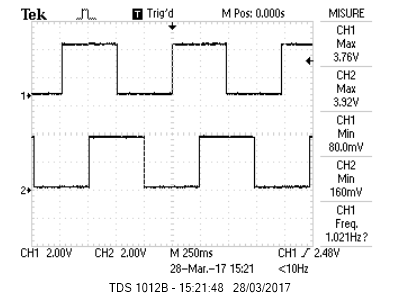
\includegraphics[scale=0.35]{../Figs-Tabs/ingressi.png}
		\label{f:ing}
	}\\
	\subfloat[acquisizione uscita porta NEND (ch2) e della tensione in ingresso A (ch1)]{
		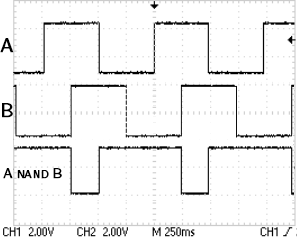
\includegraphics[scale=0.35]{../Figs-Tabs/NAND.png}
		\label{f:sci}
	}\\
	\caption{acquisizioni delle schermate impiegate per la verifica di \tablename{ \ref{t:NEND}}.}
	\label{f:osci}
\end{figure}

	Per rendere significativa l'acquisizione dell'uscita dalla porta NEND ( \figurename{ \ref{f:sci}} ) si è acquisito contemporaneamente uno dei de ingressi, nella fattispecie A; dopodiché si sono acquisiti entrambi i segnali  in ingresso (\figurename{ \ref{f:ing}} ) quale indicazione dello stato di ingresso.
	
	Dall'osservazione della \figurename{ \ref{f:osci}} si ottiene un ulteriore verifica della \tablename{ \ref{t:NEND}}.
\section{Progettazione e verifica semplici circiti logici}
	Per verificare le tabelle di verità dei seguenti circuiti si è impiegato il circuito impulsatore; ed in particolare la tecnica descritta in\textbf{ sezione \ref{sez:ard} }.
	Si segnala che per tutta la sezione verrà impiegata la \figurename{ \ref{f:ing}} quale riferimento per i segnali in ingresso.
	\subsection{AND}
	Per verificare l'andamento di un circuito AND, essendo
	$$AND(A,B) = A \cdot B = \overline{(\overline{A \cdot B})}$$
	si è montato il circuito in \figurename{ \ref{f:AND}} 
	\begin{figure}[htb]
		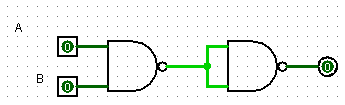
\includegraphics[scale=1.0]{../Figs-Tabs/ENd.png}
		\caption{rappresentazione di un circito AND realizzato con porte NAND. A e B rappresentano gli ingressi mentre si campiona in scita sl terzo terminale.}
	\end{figure}\label{f:AND}
.
	Tale circito presenta la tabella di verità riportata in \tablename{ \ref{t:AND}} 
	\begin{table}[htb]
		\centering
		\begin{tabular}{sss}
			\toprule
			\text{ingresso} A & \text{ingresso} B &\text{uscita porta AND }$A\cdot B$	\\
			\midrule
			0  & 0 & 0\\
			0  & 1 & 0\\
			1  & 0 & 0\\
			1  & 1 & 1\\
			\bottomrule
		\end{tabular}
		\caption{Tabella di verità di una porta AND.}
		\label{t:AND}
	\end{table}.
	la quale risulta a sua volta verificata dall'andamento osservato
	e riportato in \figurename{ \ref{f:osci-and}}
	
	\begin{figure}[hb]
		\centering
		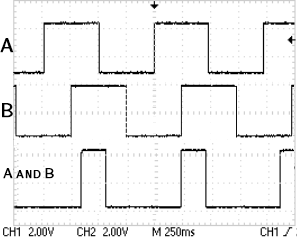
\includegraphics[scale=0.35]{../Figs-Tabs/and.png}
		\caption{acqusizione della schermata impiegata per la verifica di \tablename{ \ref{t:AND}}.
		Uscita funzione AND (ch2) e tensione in ingresso in A (ch1).
		}
		\label{f:osci-and}
	\end{figure}.
	\subsection{OR}
			Per la funzione OR essendo $$ OR(A,B) = A + B = \overline{\overline{(A +B)}}= \overline{(\overline{A} \cdot \overline{B})}$$
			è stato montato il circuito in \figurename{ \ref{f:OR}} 
		\begin{figure}[htb]
			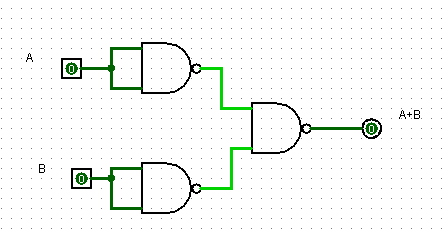
\includegraphics[scale=1.0]{../Figs-Tabs/OR2.png}
			\caption{rappresentazione di un circito OR realizzato con porte NAND. A e B rappresentano gli ingressi mentre si campiona in uscita sul terzo terminale.}
		\end{figure}\label{f:OR}.
		Tale circito presenta la tabella di verità riportata in \tablename{ \ref{t:OR}} 
		\begin{table}[htb]
			\centering
			\begin{tabular}{sss}
				\toprule
				\text{ingresso} A & \text{ingresso} B &\text{uscita porta AND }$A\cdot B$	\\
				\midrule
				0  & 0 & 0\\
				0  & 1 & 1\\
				1  & 0 & 1\\
				1  & 1 & 1\\
				\bottomrule
			\end{tabular}
			\caption{Tabella di verità di un circito OR.}
			\label{t:OR}
		\end{table}.
		la quale risulta a sua volta verificata dall'andamento osservato
		e riportato in \figurename{ \ref{f:osci-or}}
		
		\begin{figure}[hb]
			\centering
			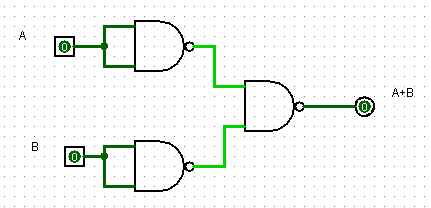
\includegraphics[scale=0.35]{../Figs-Tabs/or.png}
			\caption{acquisizione della schermata impiegata per la verifica di \tablename{ \ref{t:OR}}.
				Uscita circito OR (ch2) e tensione in ingresso in A (ch1).
			}
			\label{f:osci-or}
		\end{figure}.
	\subsection{XOR}
	Per la funzione XOR essendo $$ XOR(A,B) = A \oplus B = (A \cdot \overline{B}) + (\overline{A} \cdot B) =
	 \overline{
	 	\overline{
	 		( A \cdot \overline{
	 			(A \cdot B) )
 			}	\cdot 
 		\overline{
 			(B \cdot \overline{
 				(A \cdot B)
 			} )
 		}
 	}
	}$$
	è stato montato il circuito in \figurename{ \ref{f:XOR}} 
	\begin{figure}[htb]
		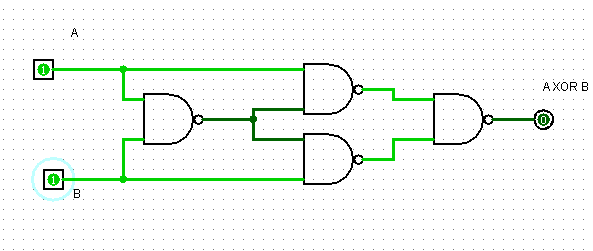
\includegraphics[scale=1.0]{../Figs-Tabs/XOR2.png}
		\caption{rappresentazione di un circuito XOR realizzato con porte NAND. A e B rappresentano gli ingressi mentre si campiona in uscita sul terzo terminale.}
	\end{figure}\label{f:XOR}.
	Tale circuito presenta la tabella di verità riportata in \tablename{ \ref{t:XOR}} 
	\begin{table}[htb]
		\centering
		\begin{tabular}{sss}
			\toprule
			\text{ingresso} A & \text{ingresso} B &\text{uscita porta XOR }$A \oplus B$	\\
			\midrule
			0  & 0 & 0\\
			0  & 1 & 1\\
			1  & 0 & 1\\
			1  & 1 & 0\\
			\bottomrule
		\end{tabular}
		\caption{Tabella di verità di un circito XOR.}
		\label{t:XOR}
	\end{table}.
	la quale risulta a sua volta verificata dall'andamento osservato
	e riportato in \figurename{ \ref{f:osci-xor}}
	
	\begin{figure}[hb]
		\centering
		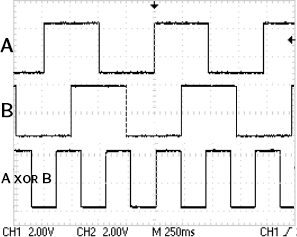
\includegraphics[scale=0.35]{../Figs-Tabs/xor.png}
		\caption{acqusizione della schermata impiegata per la verifica di \tablename{ \ref{t:XOR}}.
			Uscita circito XOR (ch2); tensione in ingresso in A (ch1).
		}
		\label{f:osci-xor}
	\end{figure}.
\subsection{Circito sommatore ad un bit}	
	Per realizzare il circuito sommatore richiesto si è assunto
	che esso potesse costituirsi su un uscita [uscita 1] di una funzione XOR, per esprimere il bit più significativo;
	ed da una funzione AND sull uscita rimanente [uscita 2] per esprimere il meno significativo.
	Si è montato pertantonto il circito in \figurename{ \ref{f:somma}}.
		\begin{figure}[htb]
		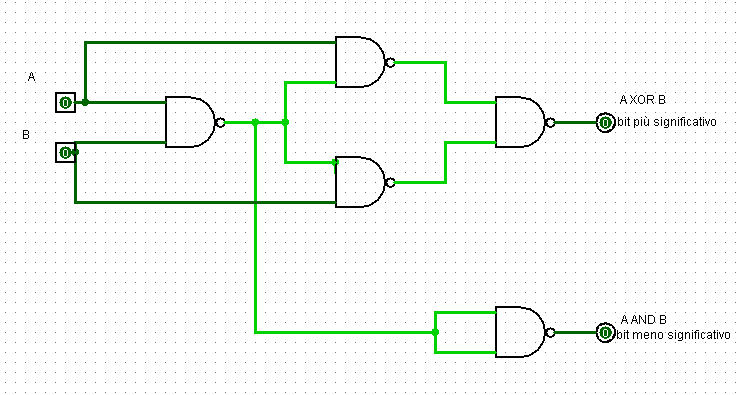
\includegraphics[scale=1.0]{../Figs-Tabs/somma.png}
		\caption{rappresentazione di un circito sommatore a 2 ingressi e 2 uscite.}
	\end{figure}\label{f:somma}
	
	L'andamento del circito risulta verificato dalla 	\figurename{ \ref{f:osci-somma}}.
	
	\begin{figure}[hb]
	\centering
	\subfloat[acqsizione della tensione in uscita dal circito XOR (ch2) ed in ingresso A (ch1);
	tale figura costituisce insieme alla \figurename{ \ref{f:ing}} un riferimento]{
		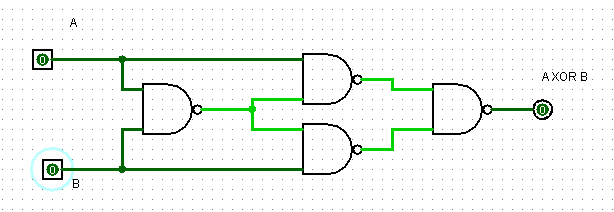
\includegraphics[scale=0.35]{../Figs-Tabs/XOR.png}
		\label{f:ing-somma}
	}\\
	\subfloat[acquisizione delle tensioni in uscita dal circito XOR (ch2) ed in uscita dal circito AND (ch1)]{
		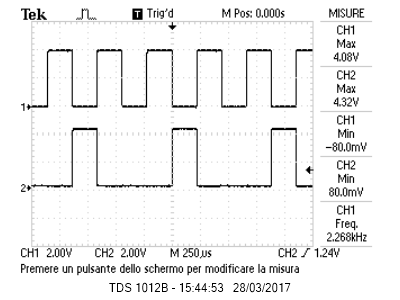
\includegraphics[scale=0.35]{../Figs-Tabs/sommatore_out.png}
		\label{f:sci-somma}
	}\\
	\caption{acqusizioni delle schermate impiegate per la verifica del funzionamento del circuito sommatore.}
	\label{f:osci-somma}
\end{figure}
Si può infatti osservare che l'uscita assuma alternativamente i valori $00-01-10-11$.


\section{Generatore di onda quadra}
	Per la realizzazione di un generatore di onda quadra
	si sono impiegati i circuiti impiegati per il multivibratore monostabile e
	per il multivibratore astabile 
	accoppiandoli in maniera da ottenere il da ottenere il circuito in \figurename{ \ref{f:qadra}}.
	\begin{figure}[htb]
		\includegraphics[scale=1.0]{../Figs-Tabs/qadra.png}
		\caption{rappresentazione del circuito realizzato per generare un onda quadra.}
	\end{figure}\label{f:qadra}

	Per il montaggio circuitale sono state impiegate le seguenti componenti\footnote{Tali valori sono stati ottenuti attraverso il multimetro digitale in dotazione. A tali misure sono state associate le incertezze calcolate sommando in quadratura l'errore di lettura con l'errore di calibrazione dello strumento.} :\\
	\begin{center}
		$R_{3}=$\SI{988 \pm 8}{\ohm}\\
		$C_{3}=$\SI{10.8 \pm 0.4 }{\nano \farad}\\
	\end{center}
	
	Si riportano in \figurename{ \ref{f:osci-qad}} l'acquisizione del segnale in 
	ingresso nel multivibratore monostabile; ovvero il segnale in uscita dal derivatore (ch2) ed il segnale in ingresso (ch1).
	\begin{figure}[htb]
		\includegraphics[scale=1.0]{../Figs-Tabs/deth_generator.png}
		\caption{Acquisizione dei segnali in ingresso [ch1] ed in uscita [ch2] dal circuito monostabile.}
	\end{figure}\label{f:osci-qad}
	Il circuito monostabile, come riscontrabile in \figurename{ \ref{f:osci-qad}},
	trasforma l'onda quadra generata dall'astabile in un impulso di breve durata temporale; sempre dalla figura in esame può essere osservato che il monostabile risulti sensibile al fronte di salita del segnale in ingresso.
	
	Come atteso, dall'andamento osservato in sezione 2, in uscita al circuito monostabile si ottiene un onda quadra [ch2 di \figurename{ \ref{f:osci-qad}}].
	Tale onda presenta un periodo 
	$T=$\SI{205 \pm 1 }{\mu \sec}
	\footnote{valori misurati con i cursori dell'oscilloscopio. Si è associata l'incertezza dovuta all'errore di posizionamento dei cursori; a cui si aggiunge a parte l'errore di calibrazione dello strumento.}
	a fronte di un impulso di $\Delta T_{up} =$\SI{47.0 \pm 0.2 }{\mu \sec}
	\footnote[1]{}
	Si ottiene pertanto un duty-cycle $\frac{\Delta T_{up}}{T}= 22.9 \pm 0.2$\textdiscount.
	
	Nella sezione 2 è stato osservato che l'impulso ,$\Delta T_{up}$, 
	abbia una dipendenza lineare dal valore della resistenza $R_{2}$;
	la durata del periodo ne risulti indipendente; poiché non varia apprezzabilmente al variare di $R_{2}$.
	
	Mentre nella sezione  è stata osservata la dipendenza lineare 
	del periodo $T$ dal valore della resistenza $R_{1}$;
	mentre la durata del impulso non vari significativamente.
	
	Si assume pertanto che $$ \Delta T_{up} \propto R_{2}$$
		$$T \propto R_{1} $$
	e non il viceversa.
	Per la verifica di tale assunzione si è proceduto a variare separatamente i valori di $R_{1}$ e $R_{2}$; si ottengono i dati in \tablename{ \ref{t:4}}.
		
	\begin{table}[htb]
		\centering
		\begin{tabular}{*{5}{S}}
			\toprule
			$R_{1}$ [\si{\ohm}] & $R_{2}$ [\si{\kilo \ohm}] & $T$ [\si{\mu \sec}] & $\Delta T_{up}$  [\si{\mu \sec}] & $\frac{\Delta T_{up}}{T}$ \\
			\midrule
			470\pm 5	&	1.12 \pm 0.01	&	234 \pm 1	&	47.6\pm2	&	4.92 \pm3	\\ 
			567 \pm6	&	1.12 \pm 0.01	&	234\pm1	&	59.2 \pm4	&	3.95\pm 0.03	\\ 
			567 \pm6	&	0.988 \pm 0.009	&	205\pm1	&	59.2 \pm0.4	&	3.46\pm0.03	\\ 
			\bottomrule
		\end{tabular}
		\caption{
			Tabella dei valori campionati per la verifica delle dipendenze di $\Delta T_{up}$ e $T$ dai valori di $R_{1}$ e  $R_{2}$.
		}
		\label{t:4}
	\end{table}
	Come possiamo osservare dai valori tabulati si ottiene un sostanziale accordo con la proporzionalità attesa.
	
	Si è adesso proceduto a realizzare un generatore di onde quadre di $T_{att}\sim 100$\si{\mu \sec} e $ \Delta {T_{up}}_{att}\sim 30$\si{\mu \sec}.
	
	Dai valori ottenuti nelle sezioni 2 e 3 e  dai rispettivi coefficienti stimati $a=$ e $b=$
		abbiamo stimato per i valori richiesti delle resistenze attese 
	${R_{2}}_{att}=$\SI{470 \pm 30}{\ohm}%valore placeholder
	${R_{1}}_{att}=$\SI{260 \pm 40}{\ohm}%valore placeholder.
	Si è osservato tuttavia che impiegando tali resistori si ottiene un impulso sensibilmente diverso da quello atteso.
	Si è pertanto proceduto a variare i valori delle resistenze sino ad ottenere un accordo tra i valori misurati e quanto richiesto.
	Al termine di tale processo sono state impiegate delle resistenze 
	$R_{1}=$\SI{331 \pm 3}{\ohm}
	$R_{2}=$\SI{464 \pm 4}{\ohm}
	ottenendo 
	$T=$\SI{101 \pm 1}{\mu \sec} e $ \Delta {T_{up}}=$\SI{30.2 \pm 0.2}{\mu \sec}.
	
	Una posssibile causa della discrepanza tra i valori dei resistori, per cui si verifichi l'accordo con le richieste, ed  i valori di ${R_{2}}_{att}$ e 	${R_{1}}_{att}$ potrebbe essere imputabile ad un andamento non esattamente lineare nelle dipendenze di $ \Delta T_{up}$ da $ R_{2}$ e di
	$T $ da $ R_{1} $
	
	
	
	
	
	
	
	
	
	
\section{Multivibratore monostabile}
\subsection{Montaggio e verifica}

Si è montato il circuito in \fig{monocazzo}, con i seguenti valori dei componenti:

\begin{figure}[H]
	\begin{minipage}{0.8\textwidth}
		\centering
		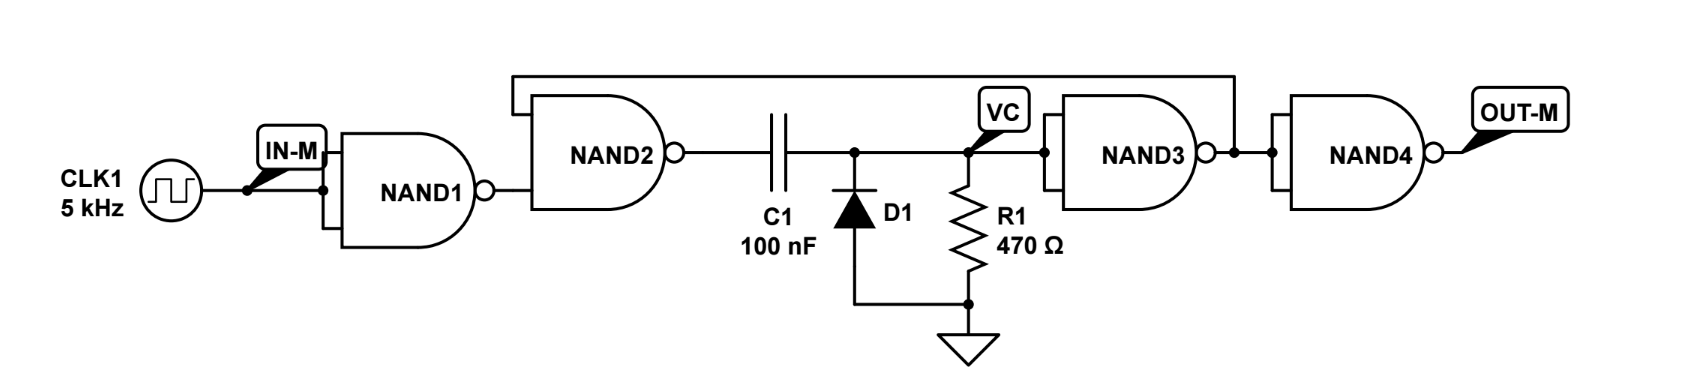
\includegraphics[scale=0.3]{monostabbo.png}
		\caption{Multivibratore monostabile.}
		\label{monocazzo}
	\end{minipage}
	\begin{minipage}{0.1\textwidth}
		\begin{tabular}{l}
			$R_1 = \SI{464(5)}{\ohm}$\\
			$C_1 = \SI{105(4)}{\nano \farad}$
		\end{tabular}
	\end{minipage}
\end{figure}

Si è verificato che il segnale in uscita fosse un onda quadra con fronte
di salita corrispondente a quello del segnale di clock in ingresso ed una durata
della semionda alta indipendente da quella del clock, come visibile in \fig{monoinout}.

\begin{figure}[H]
	\centering
	\begin{minipage}{0.3\textwidth}
		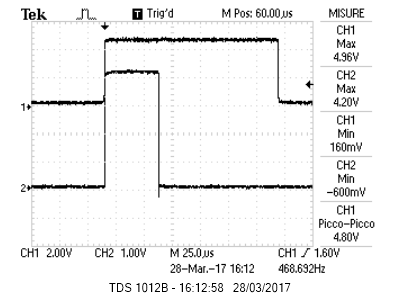
\includegraphics[scale=0.6]{monostabile_inout_500hz.png}
	\end{minipage}
	\begin{minipage}{0.3\textwidth}
		\centering
		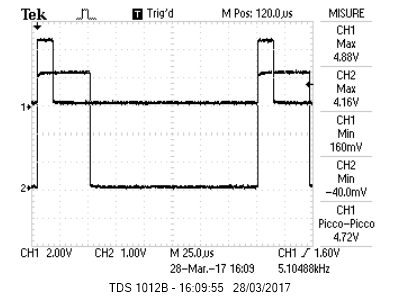
\includegraphics[scale=0.6]{monostabile_inout.png}
	\end{minipage}
	\begin{minipage}{0.3\textwidth}
		\centering
		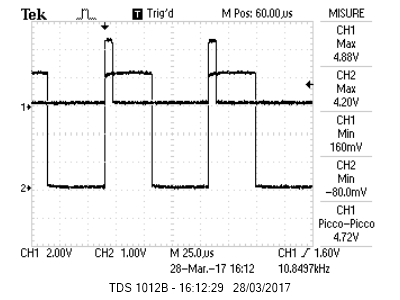
\includegraphics[scale=0.6]{monostabile_inout_10khz.png}
	\end{minipage}
	\caption{OUT-M (canale 2) e IN-M (canale 1) del multivibratore monostabile.}
	\label{monoinout}
\end{figure}

Si è dunque osservato il segnale VC in ingresso alla porta NAND3 nei due casi di
clock con semionda alta più breve e più lunga di quella del circuito
monostabile, come si riporta in \fig{monoscarica}: la tensione VC varia tra \SI{3.40(8)}{\V} e \SI{-0.64(2)}{\V}, e la commutazione del circuito avviene a  \SI{1.43(3)}{\V}.

\begin{figure}[H]
	\centering
	\begin{minipage}{0.47\textwidth}
		\centering
		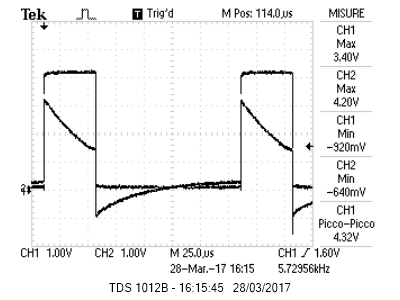
\includegraphics[scale=0.8]{monostabile_scarica.png}
	\end{minipage}
	\begin{minipage}{0.47\textwidth}
		\centering
		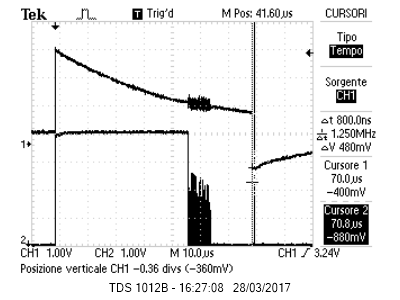
\includegraphics[scale=0.8]{monostabile_scaricaconcazzi.png}
	\end{minipage}
	\caption{OUT-M (canale 2) e VC (canale 1) del multivibratore monostabile.}
	\label{monoscarica}
\end{figure}

\subsection{Analisi del funzionamento}

In assenza di clock, il circuito mantiene output LOW: l'uscita di NAND1 è HIGH,
così come quella di NAND3, e NAND2 mantiene dunque un'uscita LOW,
ovvero prossima agli \SI{0}{\V}, e in assenza di corrente lungo $R_1$ non c'è
dunque $\Delta V$ (e di conseguenza carica) sul condensatore, cosicché anche
l'ingresso di NAND3 è LOW. Introducendo un
segnale di clock, al fronte di salita vediamo l'output di NAND1 passare a LOW e
pertanto NAND2 commuta allo stato di output HIGH: la variazione impulsiva di
tensione si trasmette attraverso il condensatore all'ingresso di NAND3, il cui
output passa dunque a LOW, portando OUT-M a HIGH. A questo punto lo stato
del clock è essenzialmente ininfluente, poiché il secondo input di NAND2 è
proprio l'output di NAND3, dunque lo stato di NAND2 non può variare fintantoché
quello di NAND3 non varia.

Poiché VC si trova ora a tensione positiva, si ha una corrente attraverso $R_1$
che porta carica sul condensatore, introducendo un $\Delta V$ ai suoi
capi e riducendo dunque la tensione a VC; quando quest'ultima scende abbastanza
da essere riconosciuta da NAND3 come un segnale LOW si ha la commutazione di
NAND3, che porta dunque allo stato LOW l'output del circuito monostabile.

In questo momento si osserva un comportamento leggermente diverso a seconda
dello stato del clock, come si osserva in \fig{monoscarica}: se il clock è già tornato LOW, la commutazione di NAND3
porta anche NAND2 a transire ad output LOW, dunque VC scende pressoché
istantaneamente ad una tensione negativa (rapidamente riportata alla tensione
di soglia del diodo dalla corrente che attraverso esso scarica velocemente il
condensatore), per poi risalire lentamente con la scarica di $C_1$ attraverso
$R_1$, e nessuna delle porte NAND cambia dunque il proprio stato.
Se al contrario il clock è ancora HIGH, e dunque l'uscita di NAND1 ancora LOW,
alla commutazione di NAND3 l'uscita di NAND2 non può passare a LOW, e il variare
di una delle due tensioni in ingresso probabilmente causa una variazione verso
l'alto della tensione in uscita, che trasmettendosi
attraverso il condensatore riporta brevemente VC sopra la soglia di
commutazione di NAND3, che dunque ritorna ad un output LOW e riporta l'uscita
di NAND2 alla tensione precedente. Questo ciclo si ripete rapidamente finché
il condensatore non si è caricato a sufficienza da mantenere VC sotto soglia
anche dopo la variazione dell'output di NAND2; quest'ultimo passerà infine a
LOW (e di conseguenza VC ad una tensione negativa) al fronte di discesa del
clock.

Il ciclo si ripete al successivo fronte di salita del clock: ci aspettiamo
dunque che il periodo del segnale del multivibratore monostabile sia pari a
quello del clock in ingresso, mentre la durata ($T_H$) dello stato HIGH
dell'output dipenda unicamente da resistenza e condensatori utilizzati.

\subsection{Linearità di $T_H$ con la resistenza}

Si è variata la resistenza $R_1$ attorno ai \SI{450}{\ohm}, misurando $T_H$, per
poi procedere ad un fit lineare $T_H = a R_1 + b$, ottenendo i seguenti risultati:

$$a = \SI{0.1095(8)}{\micro\second \per \ohm} \qquad b=\SI{-3.5(4)}{\micro \second} \qquad \chi^2/ndof = 7.0/6 \qquad corr(a,b)= -0.986$$

Dati e fit sono riportati in \fig{monofit}.

\begin{figure}[h]
	\centering
	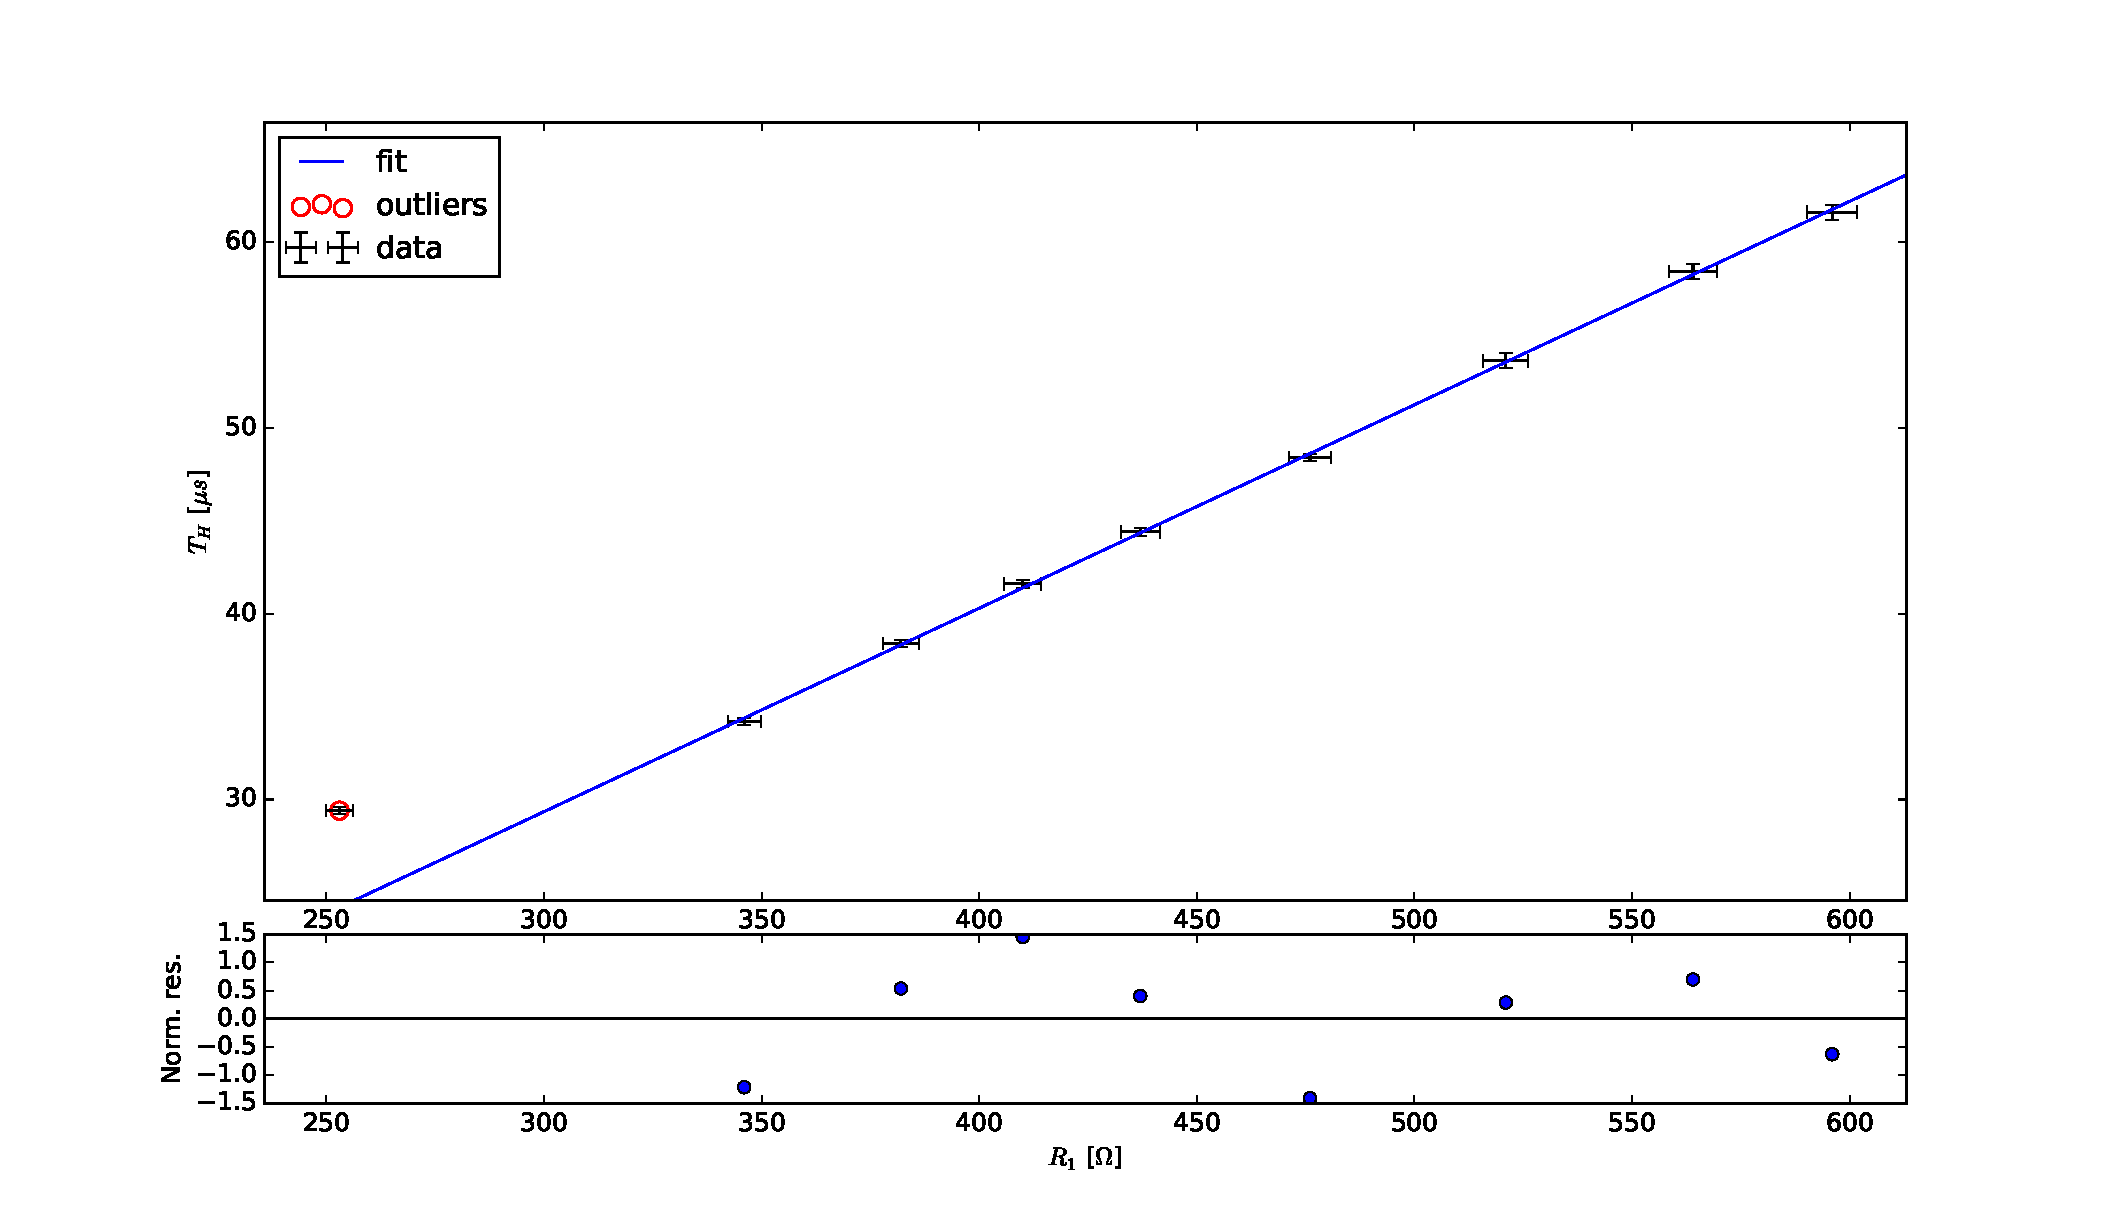
\includegraphics[scale=0.4]{monofit.pdf}
	\caption{Dati raccolti e fit della linearità del multivibratore monostabile.}
	\label{monofit}
\end{figure}

\section{Multivibratore astabile}
Si è montato il circuito in \fig{astab_sch}, con i seguenti valori dei componenti:

\begin{figure}[H]
	\begin{minipage}{0.8\textwidth}
		\centering
		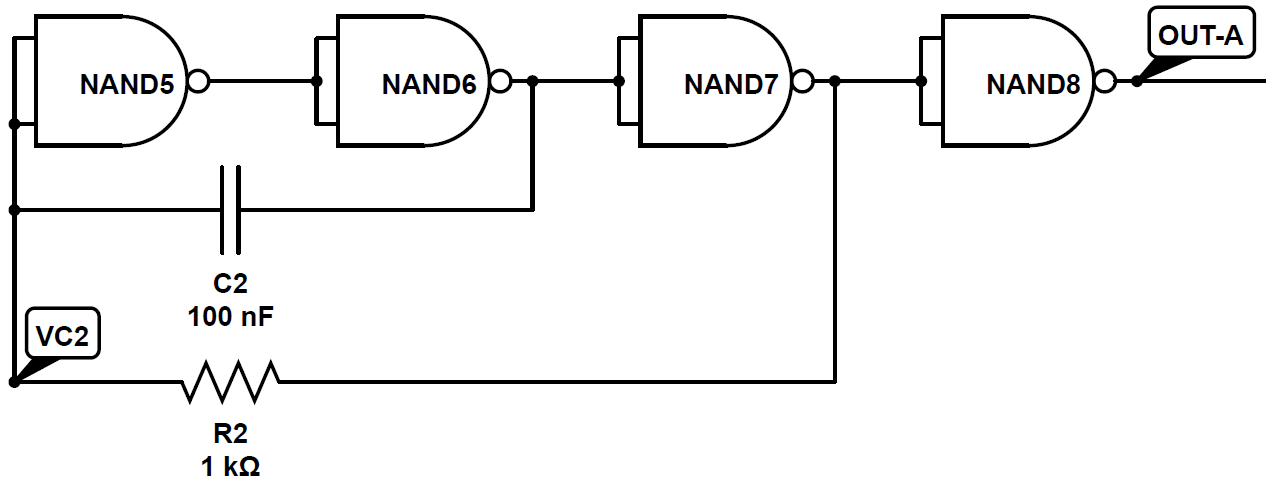
\includegraphics[scale=0.35]{astabile.png}
		\caption{Multivibratore astabile}
		\label{astab_sch}
	\end{minipage}
	\begin{minipage}{0.1\textwidth}
		\begin{tabular}{l}
			$R_2 = \SI{982(8)}{\ohm}$\\
			$C_2 = \SI{109(4)}{\nano \farad}$
		\end{tabular}
	\end{minipage}
\end{figure}

Si è verificato che il segnale in uscita fosse un onda quadra, come visibile in \fig{astab_osc} e si sono misurati periodo è duty cycle, che risultano valere:
$$T = \SI{204(1)}{\micro \second} \qquad D\% = \SI{70.1(6)}{\%}$$

\begin{figure}[H]
	\centering
	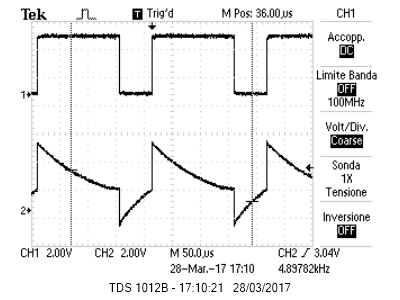
\includegraphics[scale=1]{astabile_inout.png}
	\caption{OUT-A e VC2 del multivibratore astabile}
	\label{astab_osc}
\end{figure}

Si è quindi andati ad osservare la forma d'onda all'ingresso del primo NAND (VC2), come visibile nella stessa \fig{astab_osc}.
La tensione oscilla tra \SI{4.48(12)}{\volt} e \SI{-0.68(2)}{\volt}, mentre la commutazione avviene a \SI{1.44(4)}{\volt}.

\subsection{Analisi del funzionamento}

Consideriamo un istante prima della commutazione basso/alto del NAND6 (o equivalentemente sull'uscita OUT-A): VC2 si appresta a superare $V_{comm}=\SI{1.44}{\volt}$ (la tensione di commutazione) e, essendo l'uscita del NAND6 bassa, la tensione sul condensatore è proprio uguale a VC2 ($\Delta V_C = VC_2 - V_{NAND6}$).

Raggiunta la tensione di commutazione l'uscita del NAND6 viene forzata allo stato HIGH e l'uscita del NAND7 si troverà in stato LOW, questo aumenterà istantaneamente la tensione VC2 di $V_{HIGH}=\sim \SI{3.04}{\volt}$, pari alla tensione dello stato HIGH della porta logica. Da questo punto in poi il condensatore si scaricherà con un $\tau = RC$, fino a raggiungere nuovamente la tensione di commutazione.

Nel passaggio alto/basso del NAND6 la situazione è diversa: VC2 dal valore di $\sim \SI{1.44}{\volt}$ non può diminuire oltre i $\sim\SI{-0.7}{\volt}$ per la presenza di diodi di protezione agli ingressi delle porte logiche, a questo è dovuta l'asimmetria dei semiperiodi.

Il semiperiodo HIGH è atteso essere pari a $RC\times \ln(V_{HIGH}/V_{comm}) = \SI{122(5)}{\micro\second}$, non compatibile con quello misurato di \SI{143(1)}{\micro\second}, il motivo è da ricercarsi probabilmente nel fatto che l'uscita del NAND6 non appariva costante ma aumentava leggermente nel corso del semiperiodo.
	
\subsection{Linearità del periodo con la resistenza}
Si è variata la resistenza $R_2$ in un intorno di $\SI{1000}{\ohm}$ e per ogni valore di resistenza di è misurato il periodo del segnale. I risultati raccolti sono riportati in appendice in \tab{astab_data}.
Si è quindi proceduto ad un fit lineare ($ax+b$), ottenendo i seguenti risultati:
$$a = \SI{20.74(27)}{\ohm / \micro\second} \qquad b=\SI{1.6 \pm 2.5}{\micro \second} \qquad \chi^2/ndof = 10.7/7 \qquad corr(a,b)= -0.966$$
In \fig{astab_lin} sono rappresentati i dati raccolti e il fit eseguito.

\begin{figure}[h!]
	\centering
	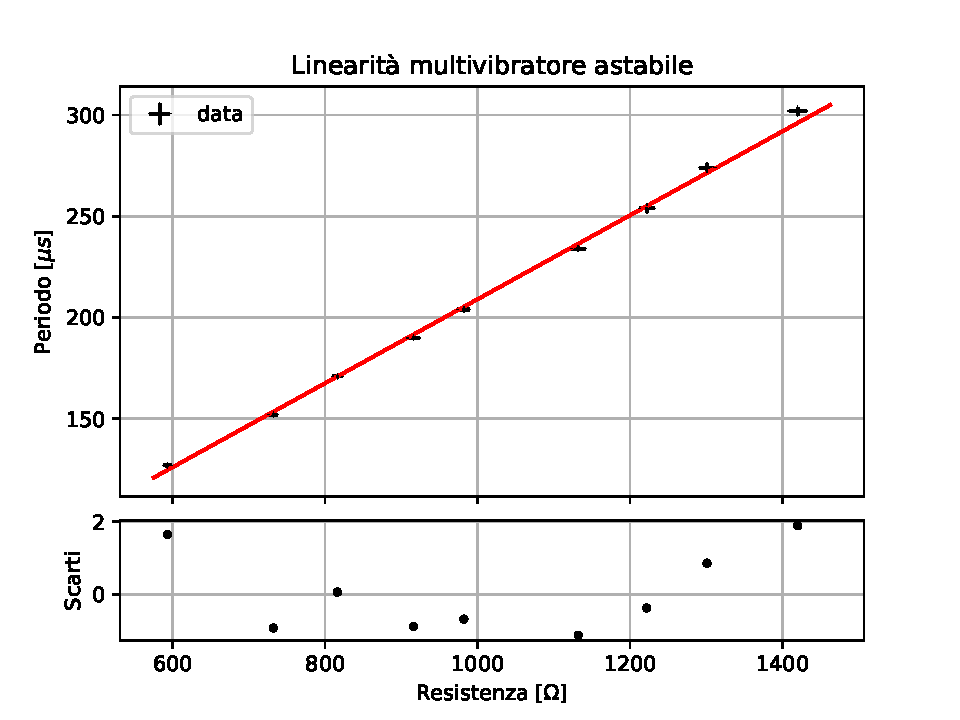
\includegraphics[scale=0.9]{fit_dati_3.pdf}
	\caption{Dati raccolti e fit della linearità del multivibratore astabile}
	\label{astab_lin}
\end{figure}





\section{Generatore di onda quadra}
	Per la realizzazione di un generatore di onda quadra si sono impiegati il multivibratore monostabile e astabile montati precedentemente, in modo da ottenere il circuito in \figurename{ \ref{f:qadra}}.

	\begin{figure}[H]
		\begin{minipage}{0.75\textwidth}
		\centering
		\includegraphics[scale=0.6]{qadra.png}
		\caption{schema del generatore di onde quadre}
		\label{f:qadra}
		\end{minipage}
		\begin{minipage}{0.14\textwidth}
			\begin{tabular}{l}
		$R_{3}=\SI{988 \pm 8}{\ohm}$\\
		$C_{3}=\SI{10.8 \pm 0.4 }{\nano \farad}$
			\end{tabular}
		\end{minipage}
	\end{figure}

	Si riporta in \figurename{ \ref{f:osci-qad}} l'acquisizione del segnale del multivibratore monostabile: il segnale in ingresso (ch1) e il segnale in uscita dal derivatore (ch2).

	\begin{figure}[H]
		\centering
		\includegraphics[scale=1.0]{deth_generator.png}
		\caption{input e output del multivibratore monostabile.}
		\label{f:osci-qad}
	\end{figure}

	Il circuito monostabile, come riscontrabile in \figurename{ \ref{f:osci-qad}},
	trasforma l'onda quadra generata dall'astabile in un impulso di breve durata temporale; sempre dalla figura in esame può essere osservato che il monostabile risulta sensibile solo al fronte di salita del segnale in ingresso.

	Come atteso in uscita al circuito monostabile si ottiene un onda quadra di periodo $T=\SI{205 \pm 1 }{\us}$ e duty cycle $D\%= 22.9 \pm 0.2$\%.

	Si è proceduto a variare separatamente i valori di $R_{1}$ e $R_{2}$, si sono ottenuti i dati in \tablename{ \ref{t:4}}.

	\begin{table}[H]
		\centering
		\begin{tabular}{cccc}
			\toprule
			$R_{1}$ [\si{\ohm}] & $R_{2}$ [\si{\kilo \ohm}] & $T$ [\si{\us}] & $\Delta T_{up}$  [\si{\us}] \\
			\midrule
			470 $\pm$ 5	&	1120 $\pm$ 10	&	234 $\pm$ 1	&	47.6 $\pm $0.2	\\
			567 $\pm$ 6	&	1120 $\pm$ 10	&	234 $\pm$ 1	&	59.2 $ \pm$ 0.4		\\
			567 $\pm$ 6	&	988 $\pm$ 9	&	205 $\pm$ 1	&	59.2 $\pm$ 0.4		\\
			\bottomrule
		\end{tabular}
		\caption{Periodo e duty cycle al variare di $R_1$ e $R_2$}
		\label{t:4}
	\end{table}

	Come possiamo osservare dai valori tabulati si osserva che la durata del semiperiodo HIGH dipende solo da $R_1$, mentre il periodo dipende solo da $R_2$.

	\paragraph{}Si è adesso proceduto a realizzare un generatore di onde quadre di $T\simeq \SI{100}{\us} $ e $D \% \simeq 30 \% $.

	Dai valori ottenuti nelle sezioni precedenti abbiamo stimato per i valori richiesti delle resistenze attese ${R_{1}}^{exp}=\SI{306(9)}{\ohm}$ e ${R_{2}}^{exp}=\SI{474 \pm 6}{\ohm}$. %R1 place holder
	% non sono riuscito a trovare il simbolo pentacolo in LaTeX, mi sembra una grave mancanza
	Si è osservato tuttavia che impiegando tali resistori si ottiene un impulso sensibilmente diverso da quello atteso, si è pertanto proceduto a variare i valori delle resistenze (per mezzo di potenziometri) sino ad ottenere i valori voluti di periodo e duty cycle.

	Al termine di tale processo sono state impiegate delle resistenze $R_{1}=$\SI{331 \pm 3}{\ohm} e $R_{2}=$\SI{464 \pm 4}{\ohm} ottenendo $T=$\SI{101 \pm 1}{\us} e $ D\%=$\SI{29.9 \pm 0.4}{\%}.

	Una causa della leggera discrepanza rispetto ai valori attesi potrebbe essere imputabile all'andamendo non esattamente lineare dei tempi con le resistenze.

\section{Appendice}
\begin{table}[hb]
	\centering
\begin{tabular}{c c} 
	\toprule
	Resistenza [$\Omega $] & Periodo [$\mu s$]\\
	\midrule
	816 $\pm$ 7 & 171 $\pm$ 1\\
	982 $\pm$ 8 & 204 $\pm$ 1\\
	593 $\pm$ 5 & 127 $\pm$ 1\\
	732 $\pm$ 6 & 152 $\pm$ 1\\
	916 $\pm$ 7 & 190 $\pm$ 1\\
	1132 $\pm$ 9 & 234 $\pm$ 1\\
	1301 $\pm$ 10 & 274 $\pm$ 2\\
	1222 $\pm$ 10 & 254 $\pm$ 2\\
	1420 $\pm$ 11 & 302 $\pm$ 2\\
	\bottomrule
\end{tabular}
\caption{Verifica della linearità nel multivibratore astabile}
	\label{astab_data}
\end{table}
\end{document}
































\section{Strmentazione}
In qest'esperienza esperienza sono state impiegate :
\begin{itemize}
	\item 2 circiti integrati SN7400 sati per costitire i circiti in esame
	\item varie resistenze e capacità impiegateanch'esse per il montaggio dei circiti
	\item 1 DIP switch a 4 interrttori
	\item 1 diodo 1N418
	\item 2 diodi LED, impiegati per rendere osservabile visivamente le tabelle di verità.
	\item Il circito implsatore basato sl Ardino nano montato nell'esperienza n:10
	\item n mltimetro digitale
	\item oscilloscopio digitale
	\item n generatore di fnzioni
\end{itemize}
\section{verifica tabella NEND}
Per la verifica della tabella di verità di na porta NEND \tablename{ \ref{t:NEND}}
\begin{table}[htb]
	\centering
	\begin{tabular}{sss}
		\toprule
		\text{ingresso} A & \text{ingresso} B &\text{scita porta NAND }$\overline{A\cdot B}$	\\
		\midrule
		0  & 0 & 1\\
		0  & 1 & 1\\
		1  & 0 & 1\\
		1  & 1 & 0\\
		\bottomrule
	\end{tabular}
	\caption{Tabella di verità di na porta NEND.}
	\label{t:NEND}
\end{table}
si è procedto in de maniere distinte; na prima verifica visiva che impiega il DIP switch in dotazione; ed na che impiega il circito implsatore basato s ardino.
Per entrambi i modi si è montato il circito in \figurename{ \ref{f:NEND}}
\begin{figure}[htb]
	\includegraphics[scale=1.0]{NEND.png}
\end{figure}\label{f:NEND}

\section{title}
\section{Strumentazione}
	In qest'esperienza esperienza sono stati impiegati :
	\begin{itemize}
		\item 2 circiti integrati SN7400 usati per costituire i circuiti in esame
		\item varie resistenze e capacità impiegate anch'esse per il montaggio dei circiti
		\item 1 DIP switch a 4 interruttori
		\item 1 diodo 1N418
		\item 2 diodi LED, impiegati per rendere osservabile visivamente le tabelle di verità. 
		\item Il circito impulsatore basato sul Arduino nano montato nell'esperienza n.10
		\item un multimetro digitale
		\item un oscilloscopio digitale 
		\item un generatore di funzioni d'onda
	\end{itemize}

\section{verifica tabella NEND}
	Per la verifica della tabella di verità di una porta NEND 
	\tablename{
		 \ref{t:NEND}
	 }
	si è proceduto in due maniere distinte. Una prima verifica visiva, che impieghi il DIP SWITCH in dotazione; 
	ed una che impieghi il circuito impulsatore basato su arduino.
	Per entrambi i modi si è montato il circuito in \figurename{ \ref{f:NEND}}.
	In tale circuito si è 
	impiegata una resistenza di pull-ups $R_{Pull-ups}=$\SI{983	\pm 8	}{\ohm} per migliorare 
	l'operatività del circito;
	una resistenza $R_{1}=$\SI{330 \pm 3 }{\ohm} montata per  limitare la richiesta di corrente al diodo.
	Il diodo LED D1 è posto in serie con $R_{1}$ e chiuso su GROUND.
	L'integrato  SN7400 è stato alimentato con una tensione di alimentazione $V_{cc}=$\SI{ 5.01 \pm 0.03  }{\volt}.
	\begin{figure}[htb]
		\includegraphics[scale=0.35]{../Figs-Tabs/NEND.png}
	\end{figure}\label{f:NEND}

\begin{table}[htb]
	\centering
	\begin{tabular}{sss}
		\toprule
		\text{ingresso} A & \text{ingresso} B &\text{uscita porta NAND }$\overline{A\cdot B}$	\\
		\midrule
		0  & 0 & 1\\
		0  & 1 & 1\\
		1  & 0 & 1\\
		1  & 1 & 0\\
		\bottomrule
	\end{tabular}
	\caption{Tabella di verità di una porta NEND.}
	\label{t:NEND}
\end{table}

\subsection{osservazione con dip switch}
	Essendo le porte NAND impiegate basate su logica TTL quando esse non risultino collegate a terra si ottiene in uscita un segnale corrispondente allo stato HIGH; cosa che non avviene qualora si abbia un collegamento a terra.
	Si è pertanto procedto a collegare da un lato gli ingressi 1 e 2 del deap switch alla tensione di GROND e da l'altro rispettivamente agli ingressi A e B del NEND.
	
	Il diodo led  essendo acceso qalora l'uscita del NEND sia alta
	e spento qualora  l'uscita sia in stato LOW
	permette la verifica della tabella di verità.
	
	Si è procedto pertanto alla verifica della tabella di verità provando le varie permitazioni degli switch 1 e 2, ottenendo n perfetto accordo con \tablename{ \ref{t:NEND}}.
\subsection{Impiego di Ardino e del oscilloscopio}\label{sez:ard}
	Per effettare una ulteriore verifica di tale tabella di verità 
	si è proceduto a collegare le porte A e B della porta NAND rispettivamente alle 
	uscite Y1 ed Y2 del circuito impulsatore, realizzato con arduino nell'esperienza 10,
	e si  collegata l'uscita della NAND all'oscilloscopio.
	
	Essendo le traccie ottente alle porte Y1 e Y2 dell'impulsatore due onde quadre 
	sfasate relativamente di $\pi/2$ su di un periodo assumono tuttue le permutazioni di due ingressi ad un bit.
	Si riportano le acquisizioni ottente all'oscilloscopio in \figurename{ \ref{f:osci}} .
	\begin{figure}[hb]
		\centering
		\subfloat[acquisizione delle tensioni in ingresso nella porta NEND; A (ch1) ed B (ch2)]{
		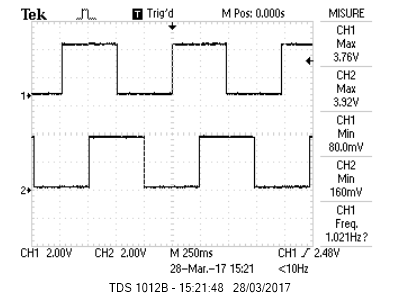
\includegraphics[scale=0.35]{../Figs-Tabs/ingressi.png}
		\label{f:ing}
	}\\
	\subfloat[acquisizione uscita porta NEND (ch2) e della tensione in ingresso A (ch1)]{
		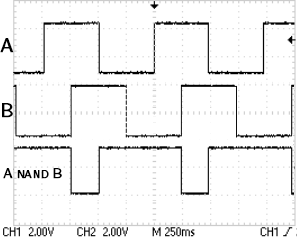
\includegraphics[scale=0.35]{../Figs-Tabs/NAND.png}
		\label{f:sci}
	}\\
	\caption{acquisizioni delle schermate impiegate per la verifica di \tablename{ \ref{t:NEND}}.}
	\label{f:osci}
\end{figure}

	Per rendere significativa l'acquisizione dell'uscita dalla porta NEND ( \figurename{ \ref{f:sci}} ) si è acquisito contemporaneamente uno dei de ingressi, nella fattispecie A; dopodiché si sono acquisiti entrambi i segnali  in ingresso (\figurename{ \ref{f:ing}} ) quale indicazione dello stato di ingresso.
	
	Dall'osservazione della \figurename{ \ref{f:osci}} si ottiene un ulteriore verifica della \tablename{ \ref{t:NEND}}.
\section{Progettazione e verifica semplici circiti logici}
	Per verificare le tabelle di verità dei seguenti circuiti si è impiegato il circuito impulsatore; ed in particolare la tecnica descritta in\textbf{ sezione \ref{sez:ard} }.
	Si segnala che per tutta la sezione verrà impiegata la \figurename{ \ref{f:ing}} quale riferimento per i segnali in ingresso.
	\subsection{AND}
	Per verificare l'andamento di un circuito AND, essendo
	$$AND(A,B) = A \cdot B = \overline{(\overline{A \cdot B})}$$
	si è montato il circuito in \figurename{ \ref{f:AND}} 
	\begin{figure}[htb]
		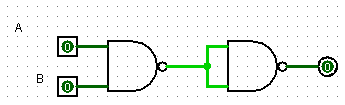
\includegraphics[scale=1.0]{../Figs-Tabs/ENd.png}
		\caption{rappresentazione di un circito AND realizzato con porte NAND. A e B rappresentano gli ingressi mentre si campiona in scita sl terzo terminale.}
	\end{figure}\label{f:AND}
.
	Tale circito presenta la tabella di verità riportata in \tablename{ \ref{t:AND}} 
	\begin{table}[htb]
		\centering
		\begin{tabular}{sss}
			\toprule
			\text{ingresso} A & \text{ingresso} B &\text{uscita porta AND }$A\cdot B$	\\
			\midrule
			0  & 0 & 0\\
			0  & 1 & 0\\
			1  & 0 & 0\\
			1  & 1 & 1\\
			\bottomrule
		\end{tabular}
		\caption{Tabella di verità di una porta AND.}
		\label{t:AND}
	\end{table}.
	la quale risulta a sua volta verificata dall'andamento osservato
	e riportato in \figurename{ \ref{f:osci-and}}
	
	\begin{figure}[hb]
		\centering
		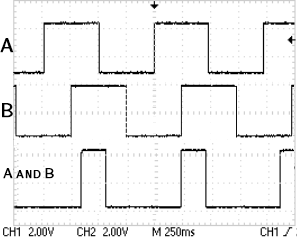
\includegraphics[scale=0.35]{../Figs-Tabs/and.png}
		\caption{acqusizione della schermata impiegata per la verifica di \tablename{ \ref{t:AND}}.
		Uscita funzione AND (ch2) e tensione in ingresso in A (ch1).
		}
		\label{f:osci-and}
	\end{figure}.
	\subsection{OR}
			Per la funzione OR essendo $$ OR(A,B) = A + B = \overline{\overline{(A +B)}}= \overline{(\overline{A} \cdot \overline{B})}$$
			è stato montato il circuito in \figurename{ \ref{f:OR}} 
		\begin{figure}[htb]
			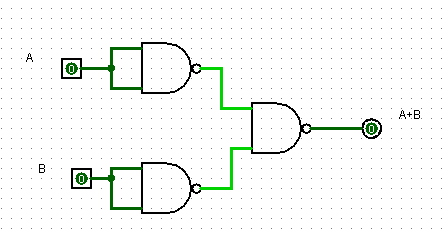
\includegraphics[scale=1.0]{../Figs-Tabs/OR2.png}
			\caption{rappresentazione di un circito OR realizzato con porte NAND. A e B rappresentano gli ingressi mentre si campiona in uscita sul terzo terminale.}
		\end{figure}\label{f:OR}.
		Tale circito presenta la tabella di verità riportata in \tablename{ \ref{t:OR}} 
		\begin{table}[htb]
			\centering
			\begin{tabular}{sss}
				\toprule
				\text{ingresso} A & \text{ingresso} B &\text{uscita porta AND }$A\cdot B$	\\
				\midrule
				0  & 0 & 0\\
				0  & 1 & 1\\
				1  & 0 & 1\\
				1  & 1 & 1\\
				\bottomrule
			\end{tabular}
			\caption{Tabella di verità di un circito OR.}
			\label{t:OR}
		\end{table}.
		la quale risulta a sua volta verificata dall'andamento osservato
		e riportato in \figurename{ \ref{f:osci-or}}
		
		\begin{figure}[hb]
			\centering
			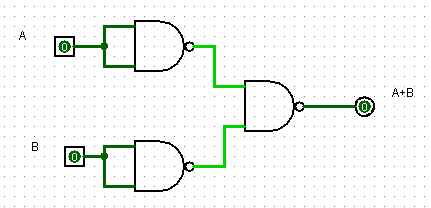
\includegraphics[scale=0.35]{../Figs-Tabs/or.png}
			\caption{acquisizione della schermata impiegata per la verifica di \tablename{ \ref{t:OR}}.
				Uscita circito OR (ch2) e tensione in ingresso in A (ch1).
			}
			\label{f:osci-or}
		\end{figure}.
	\subsection{XOR}
	Per la funzione XOR essendo $$ XOR(A,B) = A \oplus B = (A \cdot \overline{B}) + (\overline{A} \cdot B) =
	 \overline{
	 	\overline{
	 		( A \cdot \overline{
	 			(A \cdot B) )
 			}	\cdot 
 		\overline{
 			(B \cdot \overline{
 				(A \cdot B)
 			} )
 		}
 	}
	}$$
	è stato montato il circuito in \figurename{ \ref{f:XOR}} 
	\begin{figure}[htb]
		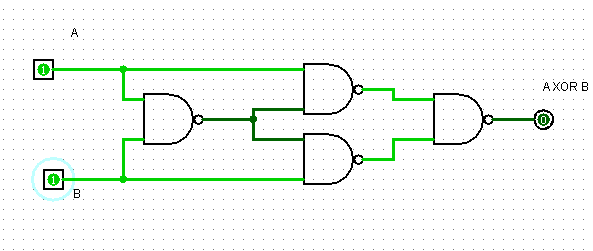
\includegraphics[scale=1.0]{../Figs-Tabs/XOR2.png}
		\caption{rappresentazione di un circuito XOR realizzato con porte NAND. A e B rappresentano gli ingressi mentre si campiona in uscita sul terzo terminale.}
	\end{figure}\label{f:XOR}.
	Tale circuito presenta la tabella di verità riportata in \tablename{ \ref{t:XOR}} 
	\begin{table}[htb]
		\centering
		\begin{tabular}{sss}
			\toprule
			\text{ingresso} A & \text{ingresso} B &\text{uscita porta XOR }$A \oplus B$	\\
			\midrule
			0  & 0 & 0\\
			0  & 1 & 1\\
			1  & 0 & 1\\
			1  & 1 & 0\\
			\bottomrule
		\end{tabular}
		\caption{Tabella di verità di un circito XOR.}
		\label{t:XOR}
	\end{table}.
	la quale risulta a sua volta verificata dall'andamento osservato
	e riportato in \figurename{ \ref{f:osci-xor}}
	
	\begin{figure}[hb]
		\centering
		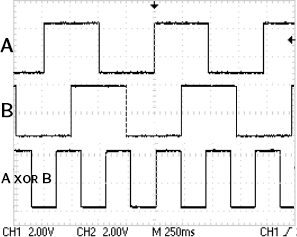
\includegraphics[scale=0.35]{../Figs-Tabs/xor.png}
		\caption{acqusizione della schermata impiegata per la verifica di \tablename{ \ref{t:XOR}}.
			Uscita circito XOR (ch2); tensione in ingresso in A (ch1).
		}
		\label{f:osci-xor}
	\end{figure}.
\subsection{Circito sommatore ad un bit}	
	Per realizzare il circuito sommatore richiesto si è assunto
	che esso potesse costituirsi su un uscita [uscita 1] di una funzione XOR, per esprimere il bit più significativo;
	ed da una funzione AND sull uscita rimanente [uscita 2] per esprimere il meno significativo.
	Si è montato pertantonto il circito in \figurename{ \ref{f:somma}}.
		\begin{figure}[htb]
		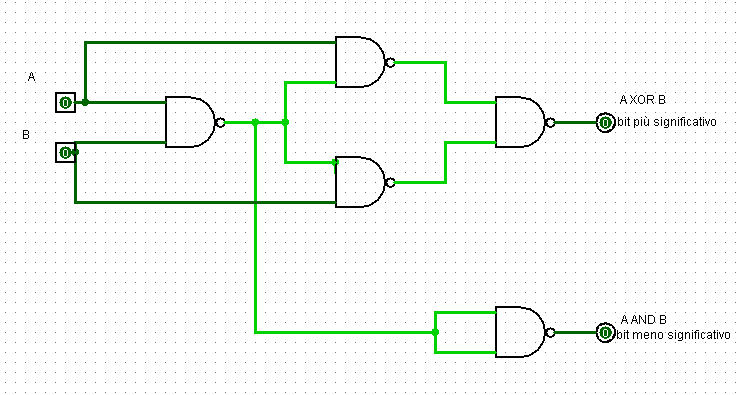
\includegraphics[scale=1.0]{../Figs-Tabs/somma.png}
		\caption{rappresentazione di un circito sommatore a 2 ingressi e 2 uscite.}
	\end{figure}\label{f:somma}
	
	L'andamento del circito risulta verificato dalla 	\figurename{ \ref{f:osci-somma}}.
	
	\begin{figure}[hb]
	\centering
	\subfloat[acqsizione della tensione in uscita dal circito XOR (ch2) ed in ingresso A (ch1);
	tale figura costituisce insieme alla \figurename{ \ref{f:ing}} un riferimento]{
		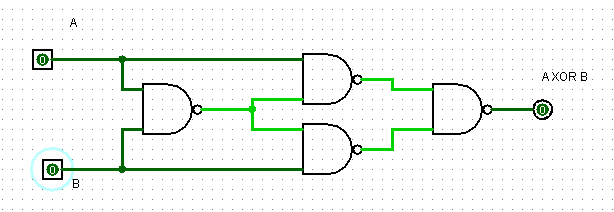
\includegraphics[scale=0.35]{../Figs-Tabs/XOR.png}
		\label{f:ing-somma}
	}\\
	\subfloat[acquisizione delle tensioni in uscita dal circito XOR (ch2) ed in uscita dal circito AND (ch1)]{
		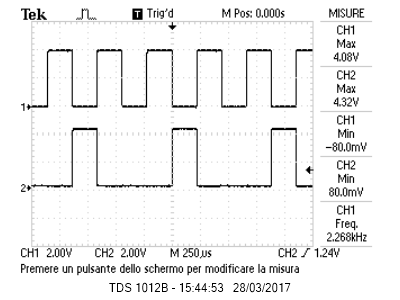
\includegraphics[scale=0.35]{../Figs-Tabs/sommatore_out.png}
		\label{f:sci-somma}
	}\\
	\caption{acqusizioni delle schermate impiegate per la verifica del funzionamento del circuito sommatore.}
	\label{f:osci-somma}
\end{figure}
Si può infatti osservare che l'uscita assuma alternativamente i valori $00-01-10-11$.


\section{Generatore di onda quadra}
	Per la realizzazione di un generatore di onda quadra
	si sono impiegati i circuiti impiegati per il multivibratore monostabile e
	per il multivibratore astabile 
	accoppiandoli in maniera da ottenere il da ottenere il circuito in \figurename{ \ref{f:qadra}}.
	\begin{figure}[htb]
		\includegraphics[scale=1.0]{../Figs-Tabs/qadra.png}
		\caption{rappresentazione del circuito realizzato per generare un onda quadra.}
	\end{figure}\label{f:qadra}

	Per il montaggio circuitale sono state impiegate le seguenti componenti\footnote{Tali valori sono stati ottenuti attraverso il multimetro digitale in dotazione. A tali misure sono state associate le incertezze calcolate sommando in quadratura l'errore di lettura con l'errore di calibrazione dello strumento.} :\\
	\begin{center}
		$R_{3}=$\SI{988 \pm 8}{\ohm}\\
		$C_{3}=$\SI{10.8 \pm 0.4 }{\nano \farad}\\
	\end{center}
	
	Si riportano in \figurename{ \ref{f:osci-qad}} l'acquisizione del segnale in 
	ingresso nel multivibratore monostabile; ovvero il segnale in uscita dal derivatore (ch2) ed il segnale in ingresso (ch1).
	\begin{figure}[htb]
		\includegraphics[scale=1.0]{../Figs-Tabs/deth_generator.png}
		\caption{Acquisizione dei segnali in ingresso [ch1] ed in uscita [ch2] dal circuito monostabile.}
	\end{figure}\label{f:osci-qad}
	Il circuito monostabile, come riscontrabile in \figurename{ \ref{f:osci-qad}},
	trasforma l'onda quadra generata dall'astabile in un impulso di breve durata temporale; sempre dalla figura in esame può essere osservato che il monostabile risulti sensibile al fronte di salita del segnale in ingresso.
	
	Come atteso, dall'andamento osservato in sezione 2, in uscita al circuito monostabile si ottiene un onda quadra [ch2 di \figurename{ \ref{f:osci-qad}}].
	Tale onda presenta un periodo 
	$T=$\SI{205 \pm 1 }{\mu \sec}
	\footnote{valori misurati con i cursori dell'oscilloscopio. Si è associata l'incertezza dovuta all'errore di posizionamento dei cursori; a cui si aggiunge a parte l'errore di calibrazione dello strumento.}
	a fronte di un impulso di $\Delta T_{up} =$\SI{47.0 \pm 0.2 }{\mu \sec}
	\footnote[1]{}
	Si ottiene pertanto un duty-cycle $\frac{\Delta T_{up}}{T}= 22.9 \pm 0.2$\textdiscount.
	
	Nella sezione 2 è stato osservato che l'impulso ,$\Delta T_{up}$, 
	abbia una dipendenza lineare dal valore della resistenza $R_{2}$;
	la durata del periodo ne risulti indipendente; poiché non varia apprezzabilmente al variare di $R_{2}$.
	
	Mentre nella sezione  è stata osservata la dipendenza lineare 
	del periodo $T$ dal valore della resistenza $R_{1}$;
	mentre la durata del impulso non vari significativamente.
	
	Si assume pertanto che $$ \Delta T_{up} \propto R_{2}$$
		$$T \propto R_{1} $$
	e non il viceversa.
	Per la verifica di tale assunzione si è proceduto a variare separatamente i valori di $R_{1}$ e $R_{2}$; si ottengono i dati in \tablename{ \ref{t:4}}.
		
	\begin{table}[htb]
		\centering
		\begin{tabular}{*{5}{S}}
			\toprule
			$R_{1}$ [\si{\ohm}] & $R_{2}$ [\si{\kilo \ohm}] & $T$ [\si{\mu \sec}] & $\Delta T_{up}$  [\si{\mu \sec}] & $\frac{\Delta T_{up}}{T}$ \\
			\midrule
			470\pm 5	&	1.12 \pm 0.01	&	234 \pm 1	&	47.6\pm2	&	4.92 \pm3	\\ 
			567 \pm6	&	1.12 \pm 0.01	&	234\pm1	&	59.2 \pm4	&	3.95\pm 0.03	\\ 
			567 \pm6	&	0.988 \pm 0.009	&	205\pm1	&	59.2 \pm0.4	&	3.46\pm0.03	\\ 
			\bottomrule
		\end{tabular}
		\caption{
			Tabella dei valori campionati per la verifica delle dipendenze di $\Delta T_{up}$ e $T$ dai valori di $R_{1}$ e  $R_{2}$.
		}
		\label{t:4}
	\end{table}
	Come possiamo osservare dai valori tabulati si ottiene un sostanziale accordo con la proporzionalità attesa.
	
	Si è adesso proceduto a realizzare un generatore di onde quadre di $T_{att}\sim 100$\si{\mu \sec} e $ \Delta {T_{up}}_{att}\sim 30$\si{\mu \sec}.
	
	Dai valori ottenuti nelle sezioni 2 e 3 e  dai rispettivi coefficienti stimati $a=$ e $b=$
		abbiamo stimato per i valori richiesti delle resistenze attese 
	${R_{2}}_{att}=$\SI{470 \pm 30}{\ohm}%valore placeholder
	${R_{1}}_{att}=$\SI{260 \pm 40}{\ohm}%valore placeholder.
	Si è osservato tuttavia che impiegando tali resistori si ottiene un impulso sensibilmente diverso da quello atteso.
	Si è pertanto proceduto a variare i valori delle resistenze sino ad ottenere un accordo tra i valori misurati e quanto richiesto.
	Al termine di tale processo sono state impiegate delle resistenze 
	$R_{1}=$\SI{331 \pm 3}{\ohm}
	$R_{2}=$\SI{464 \pm 4}{\ohm}
	ottenendo 
	$T=$\SI{101 \pm 1}{\mu \sec} e $ \Delta {T_{up}}=$\SI{30.2 \pm 0.2}{\mu \sec}.
	
	Una posssibile causa della discrepanza tra i valori dei resistori, per cui si verifichi l'accordo con le richieste, ed  i valori di ${R_{2}}_{att}$ e 	${R_{1}}_{att}$ potrebbe essere imputabile ad un andamento non esattamente lineare nelle dipendenze di $ \Delta T_{up}$ da $ R_{2}$ e di
	$T $ da $ R_{1} $
	
	
	
	
	
	
	
	
	
	
